\documentclass[tikz,border=4pt]{standalone}
\usepackage{amsmath}
\begin{document}
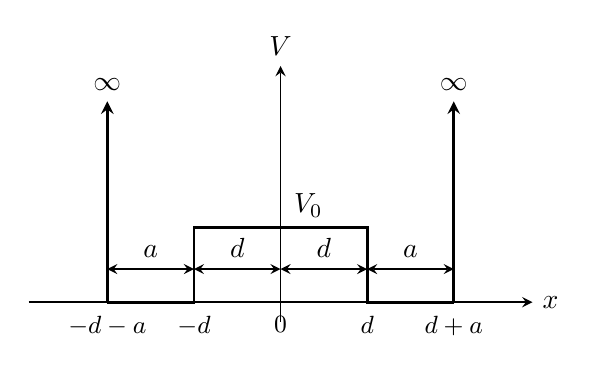
\begin{tikzpicture}[>=stealth, thick, scale=1.0]
  % Axes
  \draw[->, line width=0.65pt] (-3.2, 0) -- (3.2, 0) node[right] {$x$};
  \draw[->, line width=0.65pt] (0, -0.25) -- (0, 3.0) node[above] {$V$};

  % Potential profile: infinite walls at +-2.2, barrier width +-1.1, height 1.0
  \draw[->, line width=1.0pt] (-2.2, 0) -- (-2.2, 2.55) node[above] {$\infty$};
  \draw[->, line width=1.0pt] (2.2, 0) -- (2.2, 2.55) node[above] {$\infty$};
  \draw[line width=1.0pt] (-2.2, 0) -- (-1.1, 0) -- (-1.1, 0.95) -- (1.1, 0.95) -- (1.1, 0) -- (2.2, 0);

  % Barrier height label
  \node[above right] at (0.04, 0.95) {$V_0$};

  % Width dimension arrows: a, d, d, a
  \draw[<->, line width=0.6pt] (-2.2, 0.42) -- (-1.1, 0.42);
  \node[above] at (-1.65, 0.44) {$a$};
  \draw[<->, line width=0.6pt] (-1.1, 0.42) -- (0, 0.42);
  \node[above] at (-0.55, 0.44) {$d$};
  \draw[<->, line width=0.6pt] (0, 0.42) -- (1.1, 0.42);
  \node[above] at (0.55, 0.44) {$d$};
  \draw[<->, line width=0.6pt] (1.1, 0.42) -- (2.2, 0.42);
  \node[above] at (1.65, 0.44) {$a$};

  % Coordinate labels along x-axis
  \node[below, font=\small] at (-2.2, -0.05) {$-d-a$};
  \node[below, font=\small] at (-1.1, -0.05) {$-d$};
  \node[below, font=\small] at (0, -0.05) {$0$};
  \node[below, font=\small] at (1.1, -0.05) {$d$};
  \node[below, font=\small] at (2.2, -0.05) {$d+a$};
\end{tikzpicture}
\end{document}
